\chapter{The Major Key to Your Better Future Is You}

These notes follow a Jim Rohn seminar preserved in a curated LazyingArt LLC playlist, and they keep the surviving transcript as the primary source. The board frames are used only where they genuinely support the chapter: first as opening seminar evidence under the chalk heading \emph{Personal Dev.}, and later as evidence for a narrow plus-minus comparison around the law of use. We keep the lecture's spoken unfolding: an opening thesis, a concrete compensation puzzle, a seasonal model of life, a turn to responsibility, a move from exhortation to mechanism, then the formal laws, and finally the late sequence of goals, asking, emotional ignition, and attitude.

\section{Personal Development and the Compensation Puzzle}

Rohn begins with a paired statement, and the pairing matters. We are not given a slogan but a dependence relation and its converse. If we want more, we must become more. If we refuse change in ourselves, then the visible results remain much the same.

\begin{figure}[h]
\centering

\includegraphics[width=0.78\linewidth]{lecture_12_figure_01.png}
\caption{Opening chalkboard headed \texttt{Personal Dev.}. The board is mostly contextual evidence, but it fixes the seminar setting and the governing topic.}
\end{figure}

\begin{align}
\text{have more} &\Leftarrow \text{become more},\\
\neg(\text{change in self}) &\Rightarrow \text{same results}.
\end{align}

The lecture then adds a sharper economic heuristic:
\begin{equation}
\text{income} \not\!\!\gg \text{personal development}.
\end{equation}
This should be read exactly in the lecture's tone. It is not a formal economic theorem. It is a practical regularity: income may take a lucky jump, but unless the person grows to carry it, the money tends to drift back toward the level of the self that holds it.

From the start, then, personal development is not one subject among others. It is the master variable. Rohn reinforces this with three linked claims. Success is attracted rather than chased. The main question on the job is not only what we are getting, but what we are becoming. Happiness lies less in what we receive than in what we grow into.

\begin{align}
\text{success} &\Leftarrow \text{work on yourself},\\
\text{happiness} &\Leftarrow \text{what you become}.
\end{align}

Before he turns to the first serious puzzle, he briefly announces the evening's larger menu: basic laws, goal setting, diseases of attitude, and the day that turns a life around. That preview is worth preserving because the later lecture really does circle back to each of those promised topics.

\subsection{Question \& Answer}

\paragraph{Question.} If time is the same, what makes the difference?

\paragraph{Answer.} Value.

The lecture now narrows to compensation. Two people may work for the same company, with the same products, in the same community, under the same traffic and the same problems, and yet one makes twice as much money as the other. The puzzle is local and economic, and precisely for that reason it gives the lecture its first hard spine.

Rohn's first candidate variable is time, and he rejects it. No one gets extra time. One cannot borrow somebody else's day. Once time is held fixed, the difference-making variable must be something else.

\begin{definition}
In this lecture, \emph{value} means what a person brings to the marketplace beyond the mere passage of time. It is the operative cause of different economic results under shared conditions.
\end{definition}

The central compensation law can now be written in the lecture's own vocabulary:
\begin{align}
\text{value} &\Rightarrow \text{difference in results},\\
\text{pay} &\Leftarrow \text{value brought to marketplace},\\
\text{pay} &\not\Leftarrow \text{time alone}.
\end{align}

\paragraph{A schematic example.} Rohn asks whether, in the same time, one can become twice as valuable and make twice as much, or three times as valuable and make three times as much. Schematically, his point is:
\begin{align}
\text{same time} + \text{value} &\Rightarrow \text{pay},\\
\text{same time} + 2\times \text{value} &\Rightarrow \approx 2\times \text{pay},\\
\text{same time} + 3\times \text{value} &\Rightarrow \approx 3\times \text{pay}.
\end{align}
The symbol \(\approx\) is important here. This is not an exact pricing rule; it is a transcript-backed way of capturing the lecture's illustrative scaling claim.

The economic puzzle therefore closes by returning us to the opening thesis. It is possible to do much better at the marketplace if we go to work primarily on ourselves. The compensation question was asked in order to make that larger proposition unavoidable.

\section{The Major Key Is You}

Only after the opening thesis and the compensation puzzle does Rohn ask the audience to write down the evening's formal theme:
\begin{equation}
\text{better future} \Leftarrow \text{you}.
\end{equation}
He has them underline two words, \emph{major} and \emph{you}, because the sentence is not meant as decoration. It is meant to operate like a working axiom.

He then recounts Shoaff's abrupt lesson:
\begin{align}
\text{for things to change for you} &\Rightarrow \text{you must change},\\
\text{better life} &\Leftarrow \text{better self}.
\end{align}

What follows is one of the lecture's most important widening moves. The speaker refuses the hope that the world itself will become systematically easier. The tide comes in and goes out. It gets light and then dark. Fall is followed by winter. Some winters are hard and some easy, but winter follows fall all the same.

\subsection{Question \& Answer}

\paragraph{Question.} If life does not change, how can my life change?

\paragraph{Answer.} When we change.

This is one of the lecture's strongest formulas, and it leads directly to another:
\begin{equation}
\text{the only way it gets better for you} \Leftarrow \text{when you get better}.
\end{equation}

The point is not to deny circumstance. The point is to relocate the controllable term. Once this relocation is made, the lecture can introduce its first large model without sounding sentimental. If the world is cyclic and durable, then our problem is how to live inside its recurrence.

\section{Life as Seasons: The Four Major Lessons}

Rohn's first extended model is seasonal rather than managerial. He says that life and business are like the changing seasons, and that we cannot change the seasons but can change ourselves. This is not a decorative analogy. It is the first real pedagogy of the lecture.

\begin{equation}
\text{winter} \to \text{spring} \to \text{summer} \to \text{fall}.
\end{equation}

\begin{figure}[h]
\centering
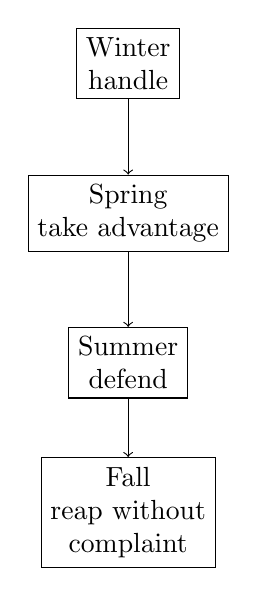
\begin{tikzpicture}[x=1cm,y=1cm]
\node[draw, align=center] (w) at (0,0) {Winter\\handle};
\node[draw, align=center] (sp) at (0,-1.9) {Spring\\take advantage};
\node[draw, align=center] (su) at (0,-3.8) {Summer\\defend};
\node[draw, align=center] (f) at (0,-5.7) {Fall\\reap without\\complaint};
\draw[->] (w.south) -- (sp.north);
\draw[->] (sp.south) -- (su.north);
\draw[->] (su.south) -- (f.north);
\end{tikzpicture}
\caption{Transcript-derived seasonal model, kept narrow and vertical for later pocket-size layout.}
\end{figure}

The lecture compresses the four lessons this way:
\begin{align}
\text{winter} &\Rightarrow \text{handle},\\
\text{spring} &\Rightarrow \text{take advantage},\\
\text{summer} &\Rightarrow \text{defend},\\
\text{fall} &\Rightarrow \text{reap without complaint}.
\end{align}

The first lesson is to handle the winters. Winter names difficulty in all its forms: recession, disappointment, panic, a broken heart, the season when one cannot figure it out. Rohn insists that winter is not removable. It is readable. January cannot be torn off the calendar; the person must instead get stronger, wiser, and better.

\begin{equation}
\text{you cannot change the seasons} \Rightarrow \text{you can change yourself}.
\end{equation}

This is why one of Shoaff's sayings enters here with great force: do not wish it were easier; wish you were better. The lecture immediately restates it twice: do not wish for fewer problems; wish for more skills. Do not wish for less challenge; wish for more wisdom.

The second lesson is to take advantage of spring. Spring is opportunity, but opportunity does not guarantee harvest. One must do something with it. Rohn puts this brutally: in life we must get good either at planting in the spring or begging in the fall. He also adds a second feature of spring, namely brevity. We receive only a handful of springs. Therefore the lecture links spring directly to reading, urgency, and the refusal to let opportunity merely pass.

The third lesson is to protect the crops all summer. Good beginnings are not left alone. Gardens are invaded. All good is attacked on this planet, and all values must be defended. Political values, marriage values, friendship values, business values, and family values all belong to the same logic. Summer is the season in which what was planted is exposed to predation, neglect, and decay.

The fourth lesson is to reap in the fall without complaint. That is the bridge from seasonal recurrence to human responsibility. If we do well, we reap without apology. If we do poorly, we reap without complaint. This is the lecture's definition of maturity at the level of harvest.

\section{Responsibility, Blame, and the Difference-Making Variable}

The seasonal model prepares the next turn exactly. If winters and springs are common events, then the crucial question becomes: what differentiates lives lived under the same happenings? Rohn answers this by way of a long blame-list. Government, taxes, prices, weather, traffic, company policy, relatives, cynical neighbors, the economy, the community: all of these appear because the lecture wants us to feel the temptation of explanation by externals.

Shoaff's interruption is the decisive cut: \emph{You ain't on it}. The self is missing from the account of failure.

\subsection{Question \& Answer}

\paragraph{Question.} What actually determines the quality of life once happenings are shared?

\paragraph{Answer.} Our response. In Rohn's repeated shorthand: what you do.

The lecture condenses the result into its second great law-like formula:
\begin{align}
\text{life quality} &\not\Leftarrow \text{what happens},\\
\text{life quality} &\Leftarrow \text{what you do}.
\end{align}

The explanatory step is clear. What happens happens to about everybody. The sun went down on all of us. Disappointments are not special gifts reserved for the poor. The same storm may confront two salesmen on the same morning, yet one stays home and the other goes out because the bad weather has emptied the roads of competitors.

\paragraph{A common-event example.} In the lecture's spirit we may write
\begin{align}
\text{same storm} + \text{stay home} &\Rightarrow \text{one result},\\
\text{same storm} + \text{go sell} &\Rightarrow \text{another result}.
\end{align}
The shared circumstance is fixed. The differing term is response.

Rohn now asks his forward-looking question: what are we going to do starting tomorrow that changes the direction of life? This transition is central. It moves us from diagnosis to mechanism, and it allows the lecture to stop sounding merely exhortative.

\section{Discipline, Study, and Learning the Setup}

Having insisted that change is possible, Rohn now asks how change is actually initiated. He first rules out two inadequate answers. It takes more than philosophical pronouncement. It takes more than enthusiasm. One may arrive at the gym excited about lifting two hundred pounds, but a second word becomes necessary there, and that word is discipline.

\begin{definition}
\emph{Discipline}, in this lecture, is the power to make oneself do the necessary things, beginning with the little disciplines that build the muscle for the larger ones.
\end{definition}

The scaling law of discipline is simple and important. Big challenges are not met by people who have never taken on the little ones. The small acts are not trivial; they are the training ground of reliable agency. Rohn makes this point by asking what we could make ourselves do starting tomorrow that would change everything.

Self-motivation follows naturally. We cannot finally hand over the work of change to somebody else. Others may teach, recruit, or encourage, but a person must motivate himself. Rohn's comic management anecdote about not sending ducks to eagle school belongs here. The point is that external systems can refine, but they cannot manufacture inward willingness.

From there the lecture tightens further:
\begin{equation}
\text{idea} \to \text{journal} \to \text{repetition} \to \text{action}.
\end{equation}
This line is not spoken as a formula on the board, but it is the lecture's actual mechanism. Ideas matter because lack of an idea, not lack of money, is the real poverty. The journal matters because the mind is not meant to serve as a filing cabinet. Repetition matters because a good idea must be revisited until it takes root and shows up in bank account, dress, personality, and lifestyle.

This is where Rohn introduces \emph{study}. If we wish to be successful, we study success; if happy, happiness; if wealthy, wealth. One studies because chance does not organize a life. Study does.

He then broadens the matter again, from study to what he calls the setup.

\begin{definition}
The \emph{setup} is Rohn's name for the law-governed arrangement of life on this planet. We did not set it up, but we are here and therefore must learn it.
\end{definition}

The lecture gives two reasons for learning the setup:
\begin{align}
\text{learn} &\Rightarrow \text{avoid harm},\\
\text{learn} &\Rightarrow \text{benefit}.
\end{align}

The first is defensive. Ignorance is not bliss; it is injury, poverty, and tragedy. The second is positive. Life is not only minus; it is also plus. If we learn the way things work, we may get on the good side of the arrangement.

Rohn also adds a crucial qualification: we do not have to like the setup, but we do have to learn it. That sentence prepares the lecture's most formal moment, because the laws are about to arrive precisely under that condition.

\section{Basic Laws: Use and Sowing}

Now the lecture becomes most equation-like. Rohn says explicitly that he is turning to the basics, and in practice that means laws. The first law is the law of use.

\begin{figure}[h]
\centering

\includegraphics[width=0.72\linewidth]{lecture_12_figure_03.png}
\caption{Plus-minus comparison on the board during the law of use. The visible layout is genuine evidence; the exact chalk wording is not fully recoverable.}
\end{figure}

The image gives us only a limited but useful fact-pattern: a minus sign on the left, a plus sign on the right, and a partially legible underlined word ending in \texttt{use}. The lecture must therefore lead the reconstruction, not the frame. The transcript gives the law in full:
\begin{equation}
\text{whatever you do not use} \Rightarrow \text{you lose}.
\end{equation}

\begin{figure}[h]
\centering
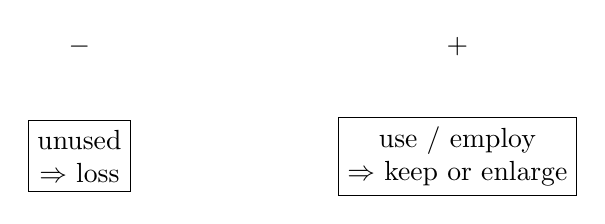
\begin{tikzpicture}[x=1cm,y=1cm]
\node at (-2.4,1.0) {$-$};
\node[draw, align=center] at (-2.4,-0.4) {unused\\$\Rightarrow$ loss};
\node at (2.4,1.0) {$+$};
\node[draw, align=center] at (2.4,-0.4) {use / employ\\$\Rightarrow$ keep or enlarge};
\end{tikzpicture}
\caption{A cautious transcript-led redraw of the visible plus-minus board comparison. The positive side is interpretive rather than directly legible.}
\end{figure}

The lecture then derives the law from a concrete bodily case. Tie the arm to the body long enough and the arm loses function. Rohn's move is then to generalize:
\begin{align}
\text{faith unused} &\Rightarrow \text{decrease},\\
\text{energy unused} &\Rightarrow \text{decrease},\\
\text{talent unused} &\Rightarrow \text{loss},\\
\text{ability unused} &\Rightarrow \text{loss}.
\end{align}

\paragraph{The logic of the law of use.} The derivation is short and characteristic.
\begin{enumerate}
\item Prevent a capacity from being exercised.
\item Leave that condition in place long enough.
\item Watch the capacity diminish or disappear.
\item Extend the same reasoning from bodily function to ambition, vitality, courage, and talent.
\end{enumerate}
The conclusion is practical rather than abstract: take a new inventory of yourself and make sure that what is present is actually being used.

\subsection{Question \& Answer}

\paragraph{Question.} What do we do with a law or arrangement we may not like?

\paragraph{Answer.} Learn it anyway: first so that we do not get hurt, and second so that we can benefit.

That answer is the bridge to the second law, the law of sowing and reaping. First it is given in the usual direction:
\begin{equation}
\text{whatever you sow} \Rightarrow \text{you reap}.
\end{equation}
Then Shoaff's crucial reversal arrives:
\begin{equation}
\text{whatever you reap} \Rightarrow \text{what you have sown}.
\end{equation}
This reversal is pedagogically decisive. It tells us where to look when the harvest disappoints. Not outward to the weather, but backward to the planting; not outward to the crowd, but inward to the mirror.

The lecture then runs through a seven-part list. Because part of that stretch is noisy in the surviving transcript, we should preserve the clearest members of the sequence:
\begin{enumerate}
\item If you sow bad, you reap bad.
\item If you sow good, you reap good.
\item You reap more than what you sow.
\item Sometimes you lose anyway.
\item If you do not sow, you do not reap.
\end{enumerate}

The third point is the most mathematically compressed:
\begin{equation}
\text{sowing} \Rightarrow \text{more than was sown}.
\end{equation}
The lecture insists that this multiplication works both ways. On the negative side:
\begin{equation}
\text{sow to the wind} \Rightarrow \text{reap the whirlwind}.
\end{equation}

The hard qualification comes later in the list and must not be omitted. One can sow well, labor honorably, tend the crop all summer, and still lose to hail the day before harvest. Rohn does not treat that as a refutation of the law. He treats it as part of the larger arrangement of the planet. The law holds inside a world where contingency still strikes.

The last secure point is equally blunt:
\begin{equation}
\text{if you do not sow} \Rightarrow \text{you do not reap}.
\end{equation}
This is why the lecture briefly turns even television time into a sowing problem: the point is not the exact arithmetic of wasted hours, but the moral that time consumed without planting leaves nothing to harvest.

\section{Goals, Reasons, Asking, and the Day of Change}

After the break, the lecture restarts with goal setting. That restart is structurally right. Once laws explain consequence, we still need chosen direction. Rohn says that reasons come first and answers second:
\begin{equation}
\text{reasons} \to \text{answers}.
\end{equation}
He means that intelligence alone does not move a life. We may be smarter than our bank balance indicates and yet remain inert because the motive structure is too weak.

The lecture then restores several motivating beats that a purely textbook chapter would lose. It gives personal reasons, family reasons, and what Rohn calls nitty-gritty reasons. The Girl Scout cookie anecdote, the Bank of America candy anecdote, the budget-finance payoff, and Bobby DePew deciding to get rich because his brother mocked him are not ornamental stories. They are case studies in how a life acquires reasons strong enough to change conduct.

Only then does the lecture formalize the goal structure:
\begin{equation}
\text{goals} = \text{long range} + \text{short range}.
\end{equation}
Long-range goals are dreams. Short-range goals are confidence builders for tomorrow, this week, this month, and this year.

\begin{figure}[h]
\centering
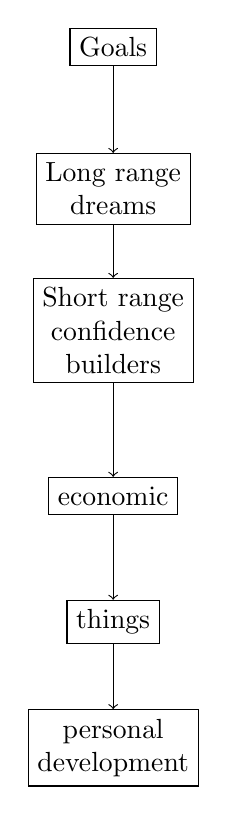
\begin{tikzpicture}[x=1cm,y=1cm]
\node[draw, align=center] (g) at (0,0) {Goals};
\node[draw, align=center] (lr) at (0,-1.8) {Long range\\dreams};
\node[draw, align=center] (sr) at (0,-3.6) {Short range\\confidence\\builders};
\node[draw, align=center] (e) at (0,-5.7) {economic};
\node[draw, align=center] (t) at (0,-7.3) {things};
\node[draw, align=center] (p) at (0,-8.9) {personal\\development};
\draw[->] (g.south) -- (lr.north);
\draw[->] (lr.south) -- (sr.north);
\draw[->] (sr.south) -- (e.north);
\draw[->] (e.south) -- (t.north);
\draw[->] (t.south) -- (p.north);
\end{tikzpicture}
\caption{Goal taxonomy kept narrow and vertical so it will survive later pocket-size export.}
\end{figure}

The short-range categories are then specified:
\begin{equation}
\text{short range goals} \supset \{\text{economic},\ \text{things},\ \text{personal development}\}.
\end{equation}

The lecture's planning law belongs immediately after this:
\begin{equation}
\text{future improves by plan, not by hope}.
\end{equation}
This is why the lecture insists on work, writing, and seriousness. One works on goals, writes them down in a journal, and examines their size and kind because goals are not passive descriptions. They affect the handshake, the personality, the gait, and the tone of the day.

\subsection{Question \& Answer}

\paragraph{Question.} Is receiving the problem?

\paragraph{Answer.} No. Failure to ask is the problem.

Rohn's asking law is one of the clearest formula clusters in the lecture:
\begin{align}
\text{ask} &\Rightarrow \text{receive},\\
\text{asking} &\Rightarrow \text{beginning of receiving},\\
\neg(\text{ask}) &\Rightarrow \text{failure to receive}.
\end{align}

The lecture then sharpens this with two images. First, asking starts a process even if we do not know the machinery behind it. Second, receiving is like the ocean: there is plenty. The problem is not that supply is gone; the problem is that some people approach the ocean with a teaspoon. Asking must therefore be done with intelligence and with faith. One makes plans like an adult and believes in them like a child.

At this point the lecture turns to the day that changes life. The sequence is emotional, but it is also structural:
\begin{equation}
\text{disgust} \to \text{decision} \to \text{desire} \to \text{resolve} \to \text{action}.
\end{equation}
Disgust says, ``I have had it.'' Decision ends inner civil war. Desire is awakened from within, often by an event one could not predict. Resolve says, ``I will,'' and Rohn finally defines it, beautifully, as promising oneself never to give up. Then comes action, because listeners are not enough; the world admires doers.

Now the lecture performs its late, surprising, but correct return to diseases of attitude. This return should not be cleaned away. Once reasons, goals, and action have been named, Rohn wants to show what can still spoil the whole enterprise.

\paragraph{Overcaution.} Life is risky all the way through. The bill for not trying may be worse than the risk of trying.

\paragraph{Pessimism.} The same measure may appear half empty or half full. The lecture does not deny difficulty; it rejects the habit of living under the exclusive jurisdiction of the bad side.

\paragraph{Thought.} Here the mental factory enters.

\begin{definition}
Rohn's \emph{mental factory} is the mind understood as a place into which thoughts pour ingredients and from which the economic, social, and personal fabric of life is built.
\end{definition}

The corresponding mental law is compact:
\begin{equation}
\text{as you think} \Rightarrow \text{so you become}.
\end{equation}

This is where the sugar and strychnine example belongs. Life contains both. It matters what falls into the coffee because it matters what enters the factory. The right ingredients support the good life; the wrong ones poison it. Hence one of Shoaff's strongest phrases: stand guard at the door of your mind.

\paragraph{Complaint.} The lecture's last disease is murmuring, whining, griping, complaining. This is not presented as mere bad manners. It is presented as a future-canceling habit. The closing Old Testament example is meant to carry exactly that warning: the good one starts must still be defended mentally.

\section{Summary}

The lecture unfolds by tightening one dependency after another. We begin with the opening pair: have more by becoming more, and expect the same results if the self does not change. The compensation puzzle then fixes value, not time, as the active economic variable. The theme card makes the matter explicit: the major key to the better future is the self. The seasons then teach us the shape of life: handle winter, use spring, defend summer, reap fall. Responsibility identifies the decisive term under shared happenings: not what happens, but what we do. Discipline, self-motivation, study, curiosity, and learning the setup supply mechanism. The law of use and the law of sowing and reaping turn the lecture most fully into equation-like reasoning. Goals, reasons, and asking give direction and pull. The emotional chain carries us into action. And the late return to overcaution, pessimism, poisoned thought, and complaint reminds us that even after the start has been made, the war is still on. The chapter therefore closes where the lecture closes: the future is not improved by waiting for the world to soften, but by the disciplined development, use, and protection of the self.